\documentclass[utf8, a4paper, 14pt, russian, oneside]{book}

% Размер шрифта
\usepackage[14pt]{extsizes}

% Кодировка
\usepackage[T2A]{fontenc}
\usepackage[utf8]{inputenc}
\usepackage[main=russian, english]{babel}

\usepackage{fontspec}
\setmainfont{Times New Roman}
\usepackage{sectsty}
\sectionfont{\large}
\subsectionfont{\large}

% Параметры страницы
\usepackage[left=3cm, right=1cm, top=2cm, bottom=2cm]{geometry}
\pagestyle{plain}
\linespread{1.1} % Межстрочный интервал

% Пакеты для работы с математикой
\usepackage{amsmath}
\usepackage{amsfonts}
\usepackage{amssymb}

% Вставка изображений
\usepackage{graphicx}

% Пакет для работы с таблицами
\usepackage{tabularx}
\usepackage{booktabs}
\usepackage{longtable}

% Для больших множеств
\usepackage{mathtools}

% Для работы с рисунками
\usepackage{caption}

% Для создания графов в 3 блоке
\usepackage[all]{xy}

% Для специальных символов
\usepackage{textcomp}

% Для гиперссылок
\usepackage{hyperref}

% Для таблиц
\usepackage{multirow}

\usepackage{upgreek}

\usepackage{array}
\newcommand{\mysec}[1]{
{\centering\section*{\hyperlink{toc}{#1}}}
\addcontentsline{toc}{section}{#1}
}

\newcommand{\mysubsec}[1]{
{\centering\subsection*{\hyperlink{toc}{#1}}}
\addcontentsline{toc}{subsection}{#1}
}

\newcommand{\Db}{
    \ensuremath{
        D_{\text{в}}
    }
}

\newcommand{\xb}{
    \ensuremath{
        x_{\text{в}}
    }
}

\newcommand{\yb}{
    \ensuremath{
        y_{\text{в}}
    }
}

\newcommand{\zb}{
    \ensuremath{
        z_{\text{в}}
    }
}

\newcommand{\yx}{
    \ensuremath{
        y_x
    }
}

\newcommand{\zx}{
    \ensuremath{
        z_x
    }
}

\newcommand{\cov}{
    \ensuremath{
        \mathit{cov}_{\text{в}}
    }
}

\renewcommand{\r}{
    \ensuremath{
        \mathit{r}_{\text{в}}
    }
}

\newcommand{\rang}{
    \ensuremath{
        \mathit{rang}
    }
}

\newcommand{\rhob}{
    \ensuremath{
        \rho_{\text{в}}
    }
}

\newcommand{\der}[2]{
    \ensuremath{
        \frac{\partial #1}{\partial #2}
    }
}

% Команды для настройки содержания
\renewcommand\contentsname{\center{Содержание}} % Вместо оглавления пишется содержание
\addto{\captionsenglish}{\renewcommand{\bibname}{References}}
\begin{document}

\thispagestyle{empty}
~\vspace{-2cm}\setlength{\parindent}{0cm}
\begin{center}
	
\includegraphics[scale=1.5]{../include/logo.png}\\[2pt]
	МИНОБРНАУКИ РОССИИ\\
	Федеральное государственное бюджетное образовательное учреждение\\
	высшего профессионального образования\\[5pt]
	\textbf{<<МИРЭА – Российский технологический университет>>}\\[5pt]
	\textbf{\large РТУ МИРЭА}\\[20pt]
	\hrule{}\mbox{}\\[1pt]
	\hrule{}\mbox{}\\[20pt]	
	Институт кибернетики \\ Кафедра <<Информационная безопасность>> (БК №252)\\[35pt]
	\textbf{Долгосрочное задание} \\
	по дисциплине: Математическая статистика
\end{center}
	\vspace{4in}
	Студент группы ККСО-01-19:  \qquad \qquad \qquad  \qquad     Колесников А.В.
\vspace{0.6in}
\begin{center}
Москва --- 2021
\end{center}
\newpage

\tableofcontents
\newpage

\mysec{Описание данных}
Среднее время круга в гонках Formula-1 c 1971 по 2020г в секундах. \footnote{http://ergast.com/mrd/db/}
\begin{table}[h!]
    \centering
    \begin{tabular}{|c|c|c|c|}
        \hline
        Год & Время & Год & Время \\ \hline
        1971 & 26,9 & 1996 & 22,5 \\ \hline
        1972 & 25,0 & 1997 & 24,7 \\ \hline
        1973 & 23,4 & 1998 & 16,9 \\ \hline
        1974 & 23,2 & 1999 & 23,1 \\ \hline
        1975 & 23,8 & 2000 & 25,1 \\ \hline
        1976 & 23,6 & 2001 & 24,5 \\ \hline
        1977 & 22,6 & 2002 & 24,2 \\ \hline
        1978 & 24,9 & 2003 & 24,0 \\ \hline
        1979 & 25,3 & 2004 & 23,2 \\ \hline
        1980 & 25,3 & 2005 & 26,3 \\ \hline
        1981 & 23,0 & 2006 & 25,7 \\ \hline
        1982 & 23,2 & 2007 & 24,3 \\ \hline
        1983 & 24,5 & 2008 & 22,7 \\ \hline
        1984 & 23,7 & 2009 & 23,9 \\ \hline
        1985 & 24,1 & 2010 & 24,8 \\ \hline
        1986 & 26,0 & 2011 & 26,4 \\ \hline
        1987 & 24,9 & 2012 & 26,2 \\ \hline
        1988 & 20,9 & 2013 & 26,3 \\ \hline
        1989 & 24,5 & 2014 & 24,2 \\ \hline
        1990 & 24,9 & 2015 & 24,1 \\ \hline
        1991 & 24,0 & 2016 & 31,7 \\ \hline
        1992 & 23,8 & 2017 & 32,0 \\ \hline
        1993 & 23,3 & 2018 & 22,6 \\ \hline
        1994 & 23,4 & 2019 & 22,8 \\ \hline
        1995 & 33,9 & 2020 & 22,6 \\ \hline
    \end{tabular}
\end{table}
\newpage

\mysec{Простейшие способы обработки статистических данных}
Порядковая статистика:
\begin{table}[h!]
    \centering
    \begin{tabular}{|c|c|c|c|c|c|c|c|c|c|}
        \hline
        20,9 & 20,9 & 22,5 & 22,6 & 22,6 & 22,6 & 22,7 & 22,8 & 23,0 & 23,1\\
        \hline
        23,2 & 23,2 & 23,3 & 23,3 & 23,4 & 23,4 & 23,6 & 23,7 & 23,8 & 23,8\\
        \hline
        23,9 & 24,0 & 24,0 & 24,1 & 24,1 & 24,2 & 24,2 & 24,3 & 24,5 & 24,5\\
        \hline
        24,5 & 24,7 & 24,8 & 24,9 & 24,9 & 24,9 & 25,0 & 25,1 & 25,3 & 25,3\\
        \hline
        25,7 & 26,0 & 26,2 & 26,3 & 26,3 & 26,4 & 28,9 & 31,7 & 33,0 & 33,9\\
        \hline
    \end{tabular}
\end{table}

Вариации:
\begin{table}[h!]
    \centering
    \begin{tabular}{|c|c|c|c|c|c|c|c|c|c|}
        \hline
        20,9 & 22,5 & 22,6 & 22,7 & 22,8 & 23,0 & 23,1 & 23,2 & 23,3 & 23,4\\
        \hline
        23,6 & 23,7 & 23,8 & 23,9 & 24,0 & 24,1 & 24,2 & 24,3 & 24,5 & 24,7\\
        \hline
        24,8 & 24,9 & 25,0 & 25,1 & 25,3 & 25,7 & 26,0 & 26,2 & 26,3 & 26,4\\
        \hline
        28,9 & 31,7 & 33,0 & 33,9 & & & & & &\\
        \hline
    \end{tabular}
\end{table}

Мода -самые частые вариации: $M_1 = 22,6; M_2 = 24,5; M_3 = 24,9$. Вариации $x_i = 22,6$, $x_i=24,5$, $x_i = 24,9$ встречаются по 3 раза.

Медина - наблюдение, стоящее в середине порядковой выборки. Поскольку объём выборки чётное число ($n=50$), то медиану посчитаем по следующей формуле:
\begin{align*}
    m = \frac{x_{\tfrac{n}{2}} + x_{\tfrac{n}{2} + 1}}{2} = \frac{24,1 + 24,2}{2} = 24,15
\end{align*}

Построим вариационный ряд:
\begin{table}[h!]
    \begin{tabular}{|c|c|c|c|c|c|c|c|c|c|c|}
        \hline
        $x_i$ & 20,9 & 22,5 & 22,6 & 22,7 & 22,8 & 23,0 & 23,1 & 23,2 & 23,3 & 23,4 \\
        \hline
        $n_i$ & 2 & 1 & 3 & 1 & 1 & 1 & 1 & 2 & 2 & 2\\
        \hline
        $w_i$ & 0,04 & 0,02 & 0,06 & 0,02 & 0,02 & 0,02 & 0,02 & 0,04 & 0,04 & 0,04 \\
        \hline
    \end{tabular}
\end{table}
\begin{table}[h!]
    \begin{tabular}{|c|c|c|c|c|c|c|c|c|c|c|}
        \hline
        $x_i$ & 23,6 & 23,7 & 23,8 & 23,9 & 24,0 & 24,1 & 24,2 & 24,3 & 24,5 & 24,7 \\
        \hline
        $n_i$ & 1 & 1 & 2 & 1 & 2 & 2 & 2 & 1 & 3 & 1 \\
        \hline
        $w_i$ & 0,02 & 0,02 & 0,04 & 0,02 & 0,04 & 0,04 & 0,04 & 0,02 & 0,06 & 0,02 \\
        \hline
    \end{tabular}
\end{table}
\newpage
\begin{table}[h!]
    \begin{tabular}{|c|c|c|c|c|c|c|c|c|c|c|}
        \hline
        $x_i$ & 24,8 & 24,9 & 25,0 & 25,1 & 25,3 & 25,7 & 26,0 & 26,2 & 26,3 & 26,4 \\
        \hline
        $n_i$ & 1 & 3 & 1 & 1 & 2 & 1 & 1 & 1 & 2 & 1 \\
        \hline
        $w_i$ & 0,02 & 0,06 & 0,02 & 0,02 & 0,04 & 0,02 & 0,02 & 0,02 & 0,04 & 0,02 \\
        \hline
    \end{tabular}
\end{table}
\begin{table}[h!]
    \begin{tabular}{|c|c|c|c|c|c|c|c|c|c|c|}
        \hline
        $x_i$ & 28,9 & 31,7 & 33,0 & 33,9\\
        \hline
        $n_i$ & 1 & 1 & 1 & 1 \\
        \hline
        $w_i$ & 0,02 & 0,02 & 0,02 & 0,02 \\
        \hline
    \end{tabular}
\end{table}

$x_i$ - значения, попавшие в выборку.\\
$n_i$ - частота вариации $x_i$.\\
$w_i$ - относительная частота вариации $x_i$.

{
\centering
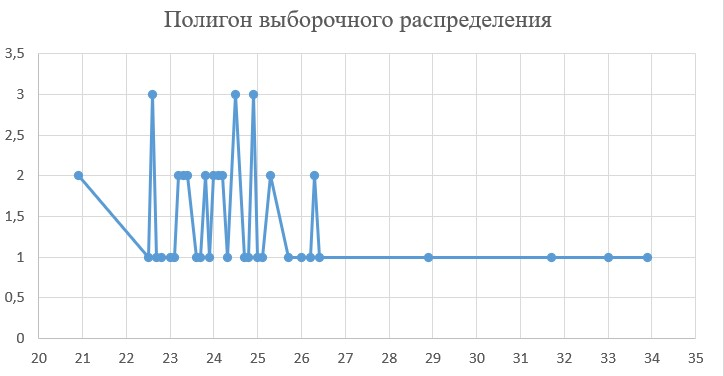
\includegraphics[scale=0.85]{img/poligon.jpg}
}

Пусть $k$ - число вариаций.

Выборочное среднее - среднее арифметическое значений выборки:
\begin{align*}
    \overline{x}_B = \sum\limits_{i=1}^{k}x_i w_i = 20,9 \cdot 0,04 + 22,5 \cdot 0,02 + \ldots + 33,9 \cdot 0,02 = 24,68.
\end{align*}

Выборочная дисперсия - мера разброса значений выборки относительно ее среднего:
\begin{align*}
    D_B(x) = \sum\limits_{i=1}^{k}x_i^2w_i - (\overline{x}_B)^2 = 20,9^2 \cdot 0,04 + \ldots + 33,9^2 \cdot 0,02 - (24,64)^2 = 6,26.
\end{align*}

Выборочное среднеквадратическое отклонение:
\begin{align*}
    \sigma_B(x) = \sqrt{{D_B(x)}} = \sqrt{6,26} = 2,5
\end{align*}
\newpage

\mysec{Доверительные интервалы}
Доверительный интервал математического ожидания при известном $\sigma_B(x)$:
\begin{align*}
    a \in \left( \overline{x}_B - t_{\gamma}\frac{\sigma}{\sqrt{n}}; \quad \overline{x}_B + t_{\gamma}\frac{\sigma}{\sqrt{n}} \right).
\end{align*}

Величина $t_{\gamma}$ находится из следующего равенства:
\begin{align*}
    2\Phi(t_\gamma) = \gamma,\  \text{где}\  \gamma\ \text{-доверительная вероятность.}
\end{align*}

Если $\gamma = 0,95,$ то $\Phi(t_\gamma) = 0,475$, а $t_\gamma = 1,96$.\\
Если $\gamma = 0,99,$ то $\Phi(t_\gamma) = 0,495$, а $t_\gamma = 2,86$.

Поскольку $\sigma = 3.1$, то при доверительной вероятности $\gamma = 0,95$ верно следующее:
\begin{align*}
    a \in \Big(24,68 - 1,96\cdot \frac{2,5}{\sqrt{50}};\  & 24,68 + 1,96\cdot \frac{2,5}{\sqrt{50}}\Big), \\
    a \in ( 23,98;\  & 25,37 ).
\end{align*}

При доверительной вероятности $\gamma=0,99$ верно:
\begin{align*}
    a \in \Big(24,68 - 2,86\cdot \frac{2,5}{\sqrt{50}};\  & 24,68 + 2,86\cdot \frac{2,5}{\sqrt{50}}\Big), \\
    a \in ( 23,67;\  & 25,69 ).
\end{align*}

Доверительный интервал математического ожидания при неизвестном $\sigma_B(x)$:
Так как $\sigma_B(x)$ неизвестно, то вычислим исправленную выборочную дисперсию:
\begin{align*}
    s^2 = \frac{n}{n-1}D_B(x) &= \frac{50}{49} \cdot 6,25 = 6,38 \\
    s = \sqrt{s^2} &= \sqrt{6,38} = 2,52 \\ 
    a \in \Big( \overline{x}_B - t_\gamma\frac{s}{\sqrt{n}};\  & \overline{x}_B + t_\gamma\frac{s}{\sqrt{n}} \Big)
\end{align*}

В данном случае $t_\gamma$ берётся из таблицы Стьюдента. $df = 50 - 1 = 49$.\\
Для $\gamma = 0,95: t_{0,95} = 2,022.$\\
Для $\gamma = 0,99: t_{0,99} = 2,680.$\\

При доверительной вероятности $\gamma=0,95$ верно:
\begin{align*}
    a \in \Big( 24,68 - 2,022 \cdot \frac{2,52}{\sqrt{50}};\  & 24,68 + 2,022 \cdot \frac{2,52}{\sqrt{50}} \Big)\\
    a \in ( 23,96;\  & 25,4).
\end{align*}

При доверительной вероятности $\gamma=0,99$ верно:
\begin{align*}
    a \in \Big( 24,68 - 2,680 \cdot \frac{2,52}{\sqrt{50}};\  & 24,68 + 2,680 \cdot \frac{2,52}{\sqrt{50}} \Big)\\
    a \in ( 23,72;\ & 25,63).
\end{align*}

Доверительный интервал дисперсии при неизвестном математическом ожидании:
\begin{align*}
    \sigma^2 \in \Bigg( \frac{(n-1)s^2}{\chi^2_{\tfrac{1+\gamma}{2},n-1}};\ & \frac{(n-1)s^2}{\chi^2_{\tfrac{1-\gamma}{2},n-1}} \Bigg)\\
    \frac{1-\gamma_1}{2} = \frac{1 - 0,95}{2} = 0,025; \quad& \frac{1+\gamma_1}{2} = \frac{1+0,95}{2} = 0,975\\
    \frac{1-\gamma_2}{2} = \frac{1 - 0,99}{2} = 0,005; \quad& \frac{1+\gamma_2}{2} = \frac{1+0,99}{2} = 0,995\\
    \chi^2_{0,975;49} = 70,22 \qquad& \chi^2_{0,025;49} = 31,55 \\
    \chi^2_{0,995;49} = 78,23 \qquad& \chi^2_{0,005;49} = 27,25
\end{align*}

При доверительной вероятности $\gamma=0,95$ верно:
\begin{align*}
    \sigma^2 \in \Big( \frac{49 \cdot 6,38}{70,22};\  & \frac{49 \cdot 6,38}{31,55} \Big)\\
    \sigma^2 \in (4,45;\  & 9,91)\\
    \sigma \in (2,11;\  & 3,15)
\end{align*}

При доверительной вероятности $\gamma=0,99$ верно:
\begin{align*}
    \sigma^2 \in \Big( \frac{49 \cdot 6,38}{78,23};\  & \frac{49 \cdot 6,38}{27,25} \Big)\\
    \sigma^2 \in (3.99;\  & 11,47)\\
    \sigma \in (1.99;\  & 3,37)
\end{align*}

\newpage

\mysec{Интервальный вариационный ряд и его характеристики}
Имеется 50 значений от 20,9 до 33,9. Пусть левая граница значения будет равна 20. Получаем отрезок [20;34].
Пусть длина интервала $h=2$.
Если значене $x_i$ попадает на границу интервалов и $x_i$ является нечётным числом, то большую часть относим к левому интервалу, в противном
случае делим попалам.
\begin{table}[h!]
    \centering
    \begin{tabular}{|c|c|c|c|c|c|c|c|}
        \hline
        $I_i$ & [20;22] & [22;24] & [24;26] & [26;28] & [28;30] & [30;32] & [32;34]\\
        \hline
        $n_i$ & 2 & 20 & 20 & 4 & 1 & 1 & 2 \\
        \hline
        $w_i$ & 0,04 & 0,4 & 0,4 & 0,08 & 0,02 & 0,02 & 0,04 \\
        \hline
    \end{tabular}
\end{table}

$I_i$ - интервал с номером $i$;\\
$n_i$ - количество вариаций $x_i$, попавших в интервал $I_i$;\\
$w_i$ - относительная частота.

\begin{center}
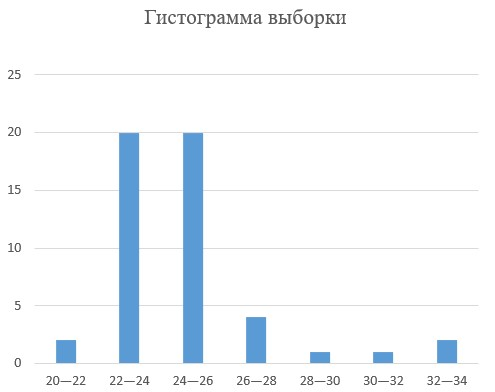
\includegraphics[scale=0.95]{img/gisto_choice.jpg}
\end{center}

Для того, чтобы определить к какой совокупности относится выборка проведём статистическую проверку.
\newpage

\mysubsec{Числовые характеристики интервального ряда}
\begin{table}[h!]
    \centering
    \begin{tabular}{|c|c|c|c|c|c|c|c|}
        \hline
        $x_i$ & 21 & 23 & 25 & 27 & 29 & 31 & 33\\
        \hline
        $n_i$ & 2 & 20 & 20 & 4 & 1 & 1 & 2 \\
        \hline
        $w_i$ & 0,04 & 0,4 & 0,4 & 0,08 & 0,02 & 0,02 & 0,04 \\
        \hline
    \end{tabular}
\end{table}

Выборочное среднее интервального ряда:
\begin{align*}
    \overline{x}_B^* = 21 \cdot 0,04 + 23 \cdot 0,4 + \ldots + 33 \cdot 0,04 = 24,72.
\end{align*}

Выборочная дисперсия интервального ряда:
\begin{align*}
    D^*_B(x) = 21^2 \cdot 0,04 + 23^2 \cdot 0,4 + \ldots + 33^2 \cdot 0,04 - (24,72)^2 = 6,08
\end{align*}

Выборочное среднеквадратическое отклонение интервального ряда:
\begin{align*}
    \sigma_B^*(x) = \sqrt{D_B^*(x)} = 2,47
\end{align*}

Функция распределения определяется вероятностью того, что случайно выбранное значение из выборки окажется меньше аргумента функции.

Выборочная функция распределения интервального ряда:
\begin{align*}
    F_n^* =
    \begin{cases}
        0   ,&\ x \leq 21, \\
        0,04,&\  21 < x \leq 23, \\
        0,44,&\  23 < x \leq 25, \\
        0,84,&\  25 < x \leq 27, \\
        0,92,&\  27 < x \leq 29, \\
        0,94,&\  29 < x \leq 31, \\
        0,96,&\  31 < x \leq 33, \\
        1   ,&\  x > 33.
    \end{cases}
\end{align*}
\newpage

\mysec{Проверка на нормальный закон распределения}
\mysubsec{Выравние частот по нормальному закону}
Предположим, что данная выборка имеет нормальный закон распределения.

Обозначим $m_i$ - выровненную по нормальному закону частоту. Найдём её по следующей формуле:
\begin{align*}
    m_i = p_i \cdot n,
\end{align*}
где $p_i = p(\alpha < x < \beta) = \Phi(\tfrac{\beta - \overline{x}_B^*}{\sigma_B^*(x)}) - \Phi(\tfrac{\alpha - \overline{x}_B^*}{\sigma_B^*(x)})$, где
$\alpha$ и $\beta$ - границы интервала, $\overline{x}_B^*$ - выборочное среднее интервального ряда, $\sigma_B^*(x)$ - среднеквадратическое отклонение.

Выпишем значения функции Лапласа для каждой границы интервалов. Напомним, что $\overline{x}_B^* = 24,72$, $\sigma_B^*(x) = 2,47$.
\begin{align*}
    \Phi \left( \frac{20 - 24,72}{2,47} \right) &= -\Phi(1,91) = -0,472,\\
    \Phi \left( \frac{22 - 24,72}{2,47} \right) &= -\Phi(1,10) = -0,365,\\
    \Phi \left( \frac{24 - 24,72}{2,47} \right) &= -\Phi(0,29) = -0,115,\\
    \Phi \left( \frac{26 - 24,72}{2,47} \right) &=  \Phi(0,52) =  0,198,\\
    \Phi \left( \frac{28 - 24,72}{2,47} \right) &=  \Phi(1,33) =  0,408,\\
    \Phi \left( \frac{30 - 24,72}{2,47} \right) &=  \Phi(2,14) =  0,483,\\
    \Phi \left( \frac{32 - 24,72}{2,47} \right) &=  \Phi(2,95) =  0,498,\\
    \Phi \left( \frac{34 - 24,72}{2,47} \right) &=  \Phi(3,76) =  0,499.
\end{align*}

Получим следующую таблицу значений:
\begin{table}[h!]
    \centering
    \begin{tabular}{|c|c|c|c|c|c|c|c|c|}
        \hline
        $\alpha_i$  & 20 & 22 & 24 & 26 & 28 & 30 & 32 & 34\\
        \hline
        $\Phi(\tfrac{\alpha_i - \overline{x}_B^*}{\sigma_B^*(x)})$ & -0,472 & -0,365 & -0,115 & 0,198 & 0,408 & 0,483 & 0,498 & 0,499\\
        \hline
    \end{tabular}
\end{table}

Для каждого интервала вычислим $p_i$:
\begin{align*}
    p_1 &= p(20 < x < 22) = -0,365 - ( -0,472 ) = 0,107, \\
    p_2 &= p(22 < x < 24) = -0,115 - ( -0,365 ) = 0,250, \\
    p_3 &= p(24 < x < 26) =  0,198 - ( -0,115 ) = 0,313, \\
    p_4 &= p(20 < x < 28) =  0,408 - (  0,198 ) = 0,210, \\
    p_5 &= p(28 < x < 30) =  0,483 - (  0,408 ) = 0,075, \\
    p_6 &= p(30 < x < 32) =  0,498 - (  0,483 ) = 0,015, \\
    p_7 &= p(32 < x < 34) =  0,499 - (  0,498 ) = 0,001 \\
\end{align*}

Получим следующую таблицу значений:
\begin{table}[h!]
    \centering
    \begin{tabular}{|c|c|c|c|c|c|c|c|c|}
        \hline
        $p_1$ & $p_2$ &$p_3$ &$p_4$ &$p_5$ &$p_6$ &$p_7$ \\
        \hline
        0,107 & 0,250 & 0,313 & 0,210 & 0,075 & 0,015 & 0,001 \\
        \hline
    \end{tabular}
\end{table}

Для каждого интервала вычислим $m_i$ - теоретическое количество попавших в $i$-ый интервал значений:
\begin{align*}
    m_1 &= 50 \cdot 0,107 = 5,35, \\
    m_2 &= 50 \cdot 0,250 = 12,5, \\
    m_3 &= 50 \cdot 0,313 = 15,65,\\
    m_4 &= 50 \cdot 0,210 = 10,5,\\
    m_5 &= 50 \cdot 0,075 = 3,75,\\
    m_6 &= 50 \cdot 0,015 = 0,75,\\
    m_7 &= 50 \cdot 0,001 = 0,05.
\end{align*}

Получим следующую таблицу значений:
\begin{table}[h!]
    \centering
    \begin{tabular}{|c|c|c|c|c|c|c|c|c|}
        \hline
        $I_i$  & [20;22] & [22; 24] & [24;26] & [26;28] & [28;30] & [30;32] & [32;34] \\
        \hline
        $n_i$ & 2 & 20 & 20 & 4 & 1 & 1 & 2 \\
        \hline
        $m_i$ & 5,35 & 12,5 & 15,65 & 10,5 & 3,75 & 0,75 & 0,05\\
        \hline
    \end{tabular}
\end{table}
\newpage

\mysubsec{Критерий $\chi^2$}
Вычислим $\chi^2_{\text{набл}}$:
\begin{align*}
    \chi^2_{\text{набл}} = \sum\limits_{i=1}^k \frac{(n_i - m_i)^2}{m_i} = \frac{(2 - 5,35)^2}{5,35} + \frac{(20 - 12,5)^2}{12,5} + \dots + \frac{(2 - 0,05)^2}{0,05} = 63,6.
\end{align*}

Из таблицы критических значений распределения $\chi^2$ найдем $\chi^2_{\text{табл}}$.
При уровне значимости $\alpha = 0,05$ и $df = k - r -1 = 7 - 2 - 1 = 4$,
где $k$ - число интервалов, $r$ - количество параметров нормального распределения. Получаем, что $\chi^2_{\text{табл}} = 9,488$.

Поскольку $\chi^2_{\text{набл}} > \chi^2_{\text{табл}}$, то не принимается гипотеза о том, что данная выборка может принадлежать генеральной совокупности
с нормальным законом распределения.

\mysubsec{Нахождение уровня значимости}

Поскольку полученное значение $\chi^2_{\text{набл}} = 63,6$ является достаточно большим и его нету в таблице квантиля распределения Пирсона, то
это значит что частоты существенно отличаются друг от друга, что и видно на графике распределения.

\mysubsec{Критерий Колмогорова}

\begin{table}[h!]
    \centering
    \begin{tabular}{|c|c|c|c|c|c|c|c|c|}
        \hline
        $I_i$  & [20;22] & [22; 24] & [24;26] & [26;28] & [28;30] & [30;32] & [32;34] \\
        \hline
        $w_i$ & 0,04 & 0,4 & 0,4 & 0,08 & 0,02 & 0,02 & 0,04 \\
        \hline
        $p_{i\text{(норм)}}$ & 0,107 & 0,250 & 0,313 & 0,210 & 0,75 & 0,015 & 0,001 \\
        \hline
    \end{tabular}
\end{table}

$F_n$ - эмпирическая функция распределения;\\
$F^*_{\text{равн}}$ - теоретическая функция равномерного распределения;\\
$F^*_{\text{норм}}$ - теоретическая функция нормального распределения;

\begin{table}[h!]
    \centering
    \begin{tabular}{|c|c|c|c|c|c|c|c|c|}
        \hline
        № интервала & 1 & 2 & 3 & 4 & 5 & 6 & 7 \\
        \hline
        $F_n(x)$ & 0,04 & 0,44 & 0,84 & 0,92 & 0,94 & 0,96 & 1 \\
        \hline
        $F^*_{\text{норм}}$ & 0,107 & 0,357 & 0,67 & 0,88 & 0,955 & 0.97 & 0,971 \\
        \hline
        $| F_n - F^*_{\text{норм}} |$ & 0,067 & 0,083 & 0,17 & 0,04 & 0,015 & 0,01 & 0,029\\
        \hline
    \end{tabular}
\end{table}
\begin{align*}
    D_{\text{норм}} &= \max{(|F_n - F^*_{\text{норм}}|)} = 0,17 \\
    \lambda_{\text{норм}} &= D_{\text{норм}} \cdot \sqrt{n} = 0,17 \cdot \sqrt{50} = 1,202\\
    P(\lambda_{\text{норм}}) &= P(1,202) = 0,1122.
\end{align*}

Вероятность того, что гипотеза о принадлежности выборки генеральной совокупности с нормальным законом распределения принята неверно, поскольку $P(\lambda_{\text{норм}}) = 0,1122$.
\newpage

\mysec{Проверка на равномерное распределение}
\mysubsec{Выравнивание частот по равномерному закону}

Предположим, что данная выборка имеет равномерный закон распределения.
Каждое являение возникает с равной вероятностью на отрезке $(a, b)$. Найдем оценки $\hat a, \hat b$ методом моментов.
\begin{table}[h!]
    \centering
    \begin{tabular}{|c|c|c|c|c|c|c|c|c|}
        \hline
        $I_i$  & [20;22] & [22; 24] & [24;26] & [26;28] & [28;30] & [30;32] & [32;34] \\
        \hline
        $n_i$ & 2 & 20 & 20 & 4 & 1 & 1 & 2 \\
        \hline
        $m_i$ & 5,35 & 12,5 & 15,65 & 10,5 & 3,75 & 0,075 & 0,05\\
        \hline
    \end{tabular}
\end{table}

\begin{align*}
    f(x) = \begin{cases}
        0, & x < a \\
        \dfrac{1}{b-a}, & a \leq x \leq b \\
        0, & x > b
    \end{cases}
\end{align*}
\begin{align*}
    \begin{cases}
        \dfrac{\hat{a} + \hat{b}}{2} = \overline{x}^*_B \\
        \dfrac{(\hat{b} - \hat{a})^2}{12} = D^*_B
    \end{cases}
    \Rightarrow
    \begin{cases}
        \hat{a} + \hat{b} = 2 \cdot \overline{x}^*_B \\
        \hat{b} - \hat{a} = 2\sqrt{3} \cdot \sigma^*_B
    \end{cases}
    \Rightarrow
    \begin{array}{l}
        \hat{b} = \overline{x}^*_B + \sqrt{3} \cdot \sigma^*_B \\
        \hat{a} = \overline{x}^*_B - \sqrt{3} \cdot \sigma^*_B \\
    \end{array}
\end{align*}

В нашем случае $\overline{x}^*_B = 24,72$, а $\sigma^*_B = 2,47$.
\begin{align*}
    \begin{array}{l}
        \hat{b} = 24,72 + \sqrt{3} \cdot 2,47 = 28,99\\
        \hat{a} = 24,72 - \sqrt{3} \cdot 2,47 = 20,44\\
    \end{array}
\end{align*}

\begin{align*}
    p_1 &= p(20 < x < 22) = \int\limits_{20}^{22}f(x) dx = \int\limits_{20,44}^{22} \frac{1}{28,99 - 20,44} dx = \\
        &= \int\limits_{20,44}^{22} 0,117 dx = 0,117 \cdot (22 - 20,44) = 0,182 \\
    p_5 &= p(28 < x < 28,99) = \int\limits_{20}^{22}f(x) dx = \int\limits_{28}^{28,99} \frac{1}{28,99 - 20,44} dx = \\
        &= \int\limits_{28}^{28,99} 0,117 dx = 0,117 \cdot (28,99 - 28) = 0,116
\end{align*}
\newpage

Аналогичным образом посчитаем остальные значения:
\begin{table}[h!]
    \centering
    \begin{tabular}{|c|c|c|c|c|}
        \hline
        $p_1$ & $p_2$ &$p_3$ &$p_4$ &$p_5$ \\
        \hline
        0,182 & 0,234 & 0,234 & 0,234 & 0,116 \\
        \hline
    \end{tabular}
\end{table}
\begin{align*}
    m_1 &= 50 \cdot p_1 = 50 \cdot 0,182 = 9,1 \\
    m_5 &= 50 \cdot p_1 = 50 \cdot 0,116 = 5,8
\end{align*}

Получим следующую таблицу:
\begin{table}[h!]
    \centering
    \begin{tabular}{|c|c|c|c|c|}
        \hline
        $m_1$ & $m_2$ &$m_3$ &$m_4$ &$m_5$ \\
        \hline
        9,1 & 11,7 & 11,7 & 11,7 & 5,8 \\
        \hline
    \end{tabular}
\end{table}
\begin{align*}
    \chi^2_{\text{набл}} = \sum\limits_{i=1}^{5} \frac{(n_i - m_i)^2}{m_i} = \frac{(2 - 9,1)^2}{9,1} + \dots + \frac{(1 - 3,75)^2}{3,75} = 26,35
\end{align*}

\mysubsec{Критерий $\chi^2$}
Из таблицы критических значений распределения $\chi^2$ найдём $\chi^2_{\text{табл}}$. При уровне значимости $\alpha = 0,05$ и $df = k - r - 1 = 5 - 2 - 1 = 2$,
где $k$ - число интервалов, $r$ - количество параметров нормального распределения. Получим, что $\chi^2_{\text{табл}} = 5,991$.

Поскольку, $\chi^2_{\text{набл}} > \chi^2_{\text{табл}}$, следовательно не принимается гипотеза о том, что данная выборка может принадлежать генеральной совокупности
с равномерным законом распределения.

\mysubsec{Нахождение уровня значимости}

Поскольку $\chi^2_{\text{набл}} = 26,35$ нет в таблице при уровне свободы $df=2$, и значение является достаточно большим, то это свидетельствует о существенном различии между частотами распределения.

\mysubsec{Критерий Колмогорова}

\begin{table}[h!]
    \centering
    \begin{tabular}{|c|c|c|c|c|c|c|c|c|}
        \hline
        $I_i$  & [20;22] & [22; 24] & [24;26] & [26;28] & [28;30] \\
        \hline
        $w_i$ & 0,04 & 0,4 & 0,4 & 0,08 & 0,02 \\
        \hline
        $p_{i(\text{равн})}$ & 0,182 & 0,234 & 0,234 & 0,234 & 0,116 \\
        \hline
    \end{tabular}
\end{table}

\begin{table}[h!]
    \centering
    \begin{tabular}{|c|c|c|c|c|c|c|c|c|}
        \hline
        № интервала & 1 & 2 & 3 & 4 & 5 \\
        \hline
        $F_n(x)$ & 0,04 & 0,44 & 0,84 & 0,92 & 0,94 \\
        \hline
        $F^*_{\text{норм}}$ & 0,182 & 0,416 & 0,65 & 0,883 & 1 \\
        \hline
        $| F_n - F^*_{\text{норм}} |$ & 0,142 & 0,024 & 0,19 & 0,037 & 0,06 \\
        \hline
    \end{tabular}
\end{table}
\begin{align*}
    D_{\text{норм}} &= \max{(|F_n - F^*_{\text{норм}}|)} = 0,142 \\
    \lambda_{\text{норм}} &= D_{\text{норм}} \cdot \sqrt{n} = 0,142 \cdot \sqrt{50} = 1,004\\
    P(\lambda_{\text{норм}}) &= P(1,004) = 0,27.
\end{align*}

Таким образом, вероятность того, что гипотеза о принадлежности выборки генеральной совокупности с равномерным распределением принята неверно, поскольку $P(\lambda_{\text{(равн)}}) = 0,27$.

\newpage
\mysec{Вычисление выборочного коэффициента асимметрии и эксцесса}

Ассиметрия показывает сдвиг пика гистограммы выборки по оси абсцисс относительно стандартного нормального распределения.
\begin{align*}
    \alpha_{SB} = \frac{
        \frac{1}{n} \sum_{i=1}^{k}(x_i - \overline{x}_B)^3 \cdot n_i
    }{\sigma_B^3(x)}    
\end{align*}
$x_i$ - середина $i$-го интервала;\\
$\overline{x}_B$ - выборочное среднее интервального ряда;\\
$\sigma_B(x)$ - среднеквадратическое отклонение интервального ряда;\\
$n$ - объём выборки;\\
$n_i$ - число значений, входящих в $i$-й интервал.

\begin{align*}
    a_{SB} = \frac{(21 - 24,72)^3 \cdot 2 + \ldots + (33 - 24,72)^3 \cdot 2}{50 \cdot 2,47^3} = 1,73.
\end{align*}
Ассиметрия данной выборки больше нуля, значит, её значения смещены вправо.

Эксцесс показывает сжатость гистограммы выборки относительно нормального распределения:
\begin{align*}
    l_{SB} = \frac{
        \frac{1}{n} \sum_{i=1}^{k}(x_i - \overline{x}_B)^4 \cdot n_i
    }{\sigma_B^4(x)}
    - 3
\end{align*}
\begin{align*}
    l_{SB} = \frac{(21 - 24,72)^4 \cdot 2 + \ldots + (33 - 24,72)^4 \cdot 2}{50 \cdot 2,47^4} = 6,42.
\end{align*}

Эксцесс данной выборки больше нуля, следовательно, график распределения выборки более сжатый, чем график нормального распределения.

\newpage

\mysec{Вывод}
В результате проведенных вычислений можно сделать следующие выводы.

Среднее время круга в гонках Formula-1 в период с 1971 по 2020 гг. примерно равно 24,7 секунды. Судя по полученным вычисления, сделать однозначный вывод
о том, какому распределению принадлежит данная выборка не удалось, поскольку значения сильно отличаются, что показывает $\chi^2$.

Но в то же время критерий Колмогорова показал, что данная выборка всё же больше относится к равномерному распределению, нежели нормальному поскольку
$P(\lambda_{норм}) = 0,1122 < P(\lambda_{\text{равн}}) = 0,27$. Поскольку $\chi^2$ получилось достаточно большим в обоих случаях это может свидетельствовать 
о существенном разбросе частот.

Ассиметрия показывает, что пик гистограммы выборки по оси абсцисс смещён правее относительно нормального распределения.
Коэффицент эксцесса показывает, что график распределения выборки более сжатый, чем график нормального распределения.

\end{document}